%Local preamble

\newcommand{\drawtestimages}[3]{%
% 1: true label: e.g. Urban100
% 2: root image : project-urban-100
% 3: scale
    \begin{figure}
        \begin{subfigure}{0.5\textwidth}
            \centering
            \includegraphics[scale=#3]{#2-input-denorm}
            \caption{Input}
        \end{subfigure}
        \begin{subfigure}{0.5\textwidth}
            \centering
            \includegraphics[scale=#3]{#2-gt-denorm}
            \caption{Ground truth.}
        \end{subfigure}
        \begin{subfigure}{0.33\textwidth}
            \centering
            \includegraphics[scale=#3]{#2-bicubic-denorm}
            \caption{Bicubic.}
        \end{subfigure}
        \begin{subfigure}{0.33\textwidth}
            \centering
            \includegraphics[scale=#3]{#2-output-denorm}
            \caption{Output base model.}
        \end{subfigure}
        \begin{subfigure}{0.33\textwidth}
            \centering
            \includegraphics[scale=#3]{#2-output-average}
            \caption{Output ensemble model.}
        \end{subfigure}
        \caption{Base model applied to #1.}\label{project:test-#1}
    \end{figure}
}

\section{Project}

\subsection{Hardware}
The following hardware was used:
\begin{itemize}
    \item GTX1060 (6 GB)
\end{itemize}

\subsection{Architecture configuration}
\begin{figure}
    \begin{subfigure}{\textwidth}
        \centering
        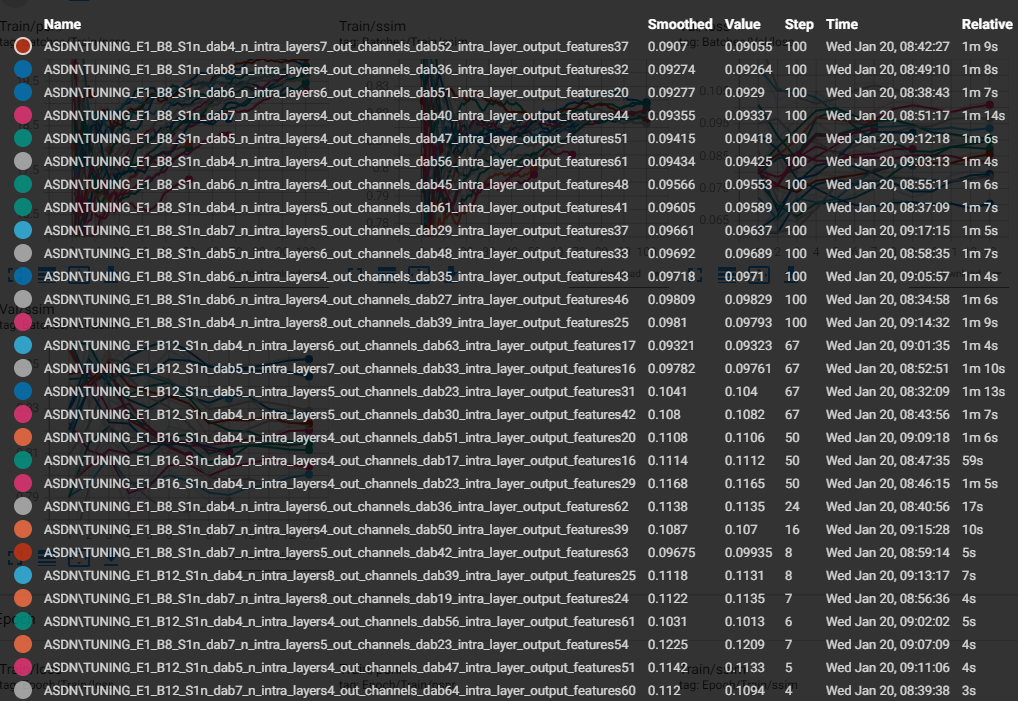
\includegraphics[width=\textwidth, keepaspectratio]{project-tuning-random-configs.png}
        \caption{Training time of different random configurations. There are many other configurations missing due to \textit{out of memory} error.}\label{project:random-configurations}
    \end{subfigure}
    \begin{subfigure}{\textwidth}
        \centering
        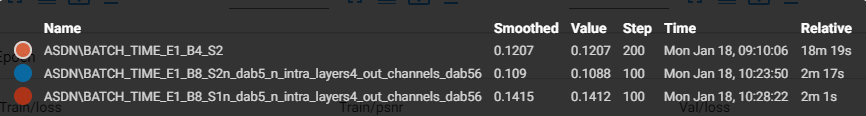
\includegraphics[width=\textwidth, keepaspectratio]{project-tuning-batch-time.png}        
        \caption{Comparison between the training time of 1 epoch of the default configuration, using the trick and not using the trick.}\label{project:batch-time}
    \end{subfigure}

    \caption{Trining time of 1 epoch. The name contains: E is \textit{epoch}, B is \textit{batch size}, S is \textit{save checkpoint} and the network parameters.}    
\end{figure}

\textbf{ASDN} is using a bi-dense connection this means a lot of memory is used for storing intermediate activations as well as gradients: the default configuration, number of dense attention block 16 and number of intra connected layers 8, is not suitable for my computer.

In order to train the default configuration an implementation trick can be used (\textbf{save checkpoint}\footnote{\href{https://pytorch.org/docs/stable/checkpoint.html}{PyTorch checkpoint}}): avoid to store gradient and activations during the forward pass and recompute them during the backward pass; but this increase the training time of a \textbf{single batch} as we can see from \Cref{project:batch-time}

Among many configurations tried [\Cref{project:random-configurations}] the final configuration chosen uses half the parameters with respect to the default configuration:

\begin{tabular}{lcc}
    & Project architecture & Paper architecture \\
    DABs & 8 & 16 \\
    IDBs & 4 & 8 \\
    Features DAB & 32 & 64 \\
    Features IDB & 32 & 64 
\end{tabular}

\subsection{Experiments}

\subsubsection{The initial LR}

\begin{figure}[h]
    \begin{subfigure}{\textwidth}
        \centering
        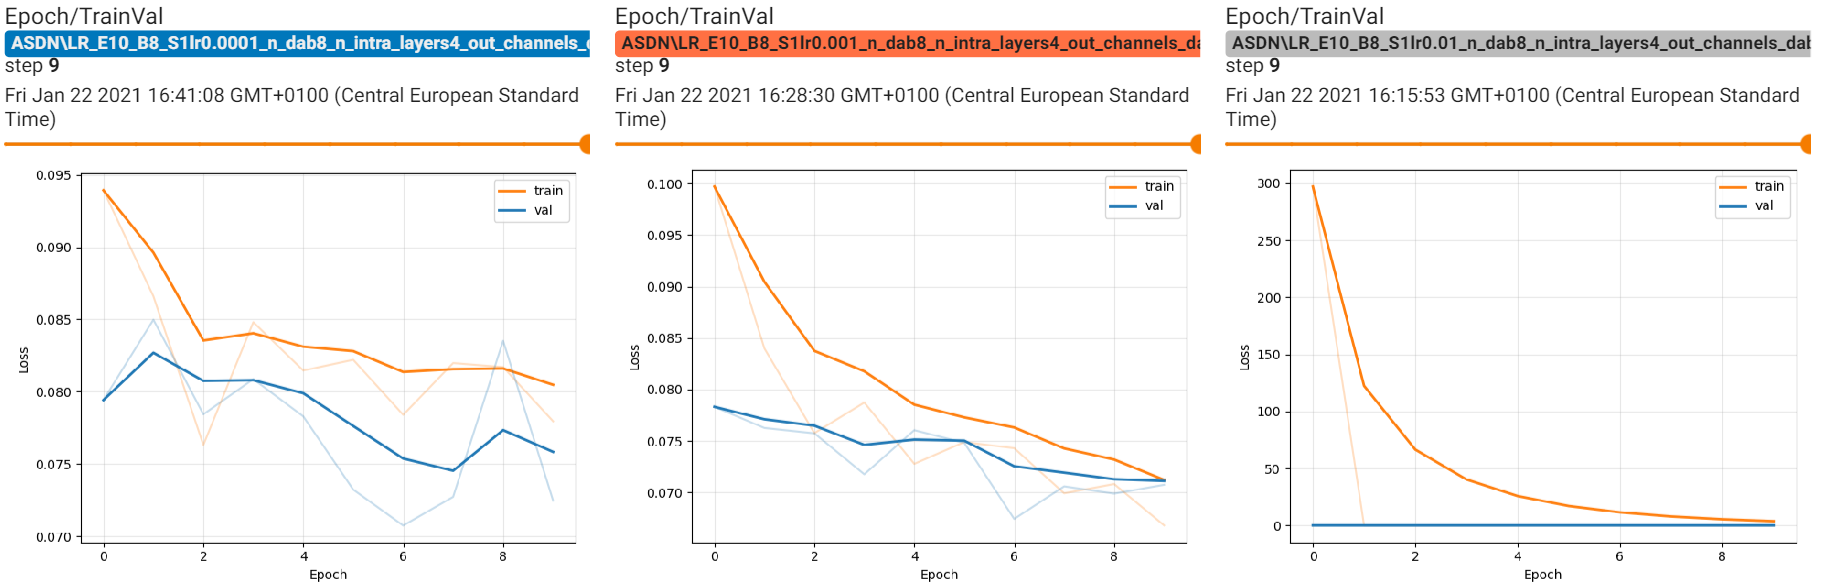
\includegraphics[width=\textwidth, keepaspectratio]{project-train-val-loss-lr.png}
        \caption{Loss values with lr: 0.01 (right), 0.001(middle), 0.0001(left)}
    \end{subfigure}
    \begin{subfigure}{\textwidth}
        \centering
        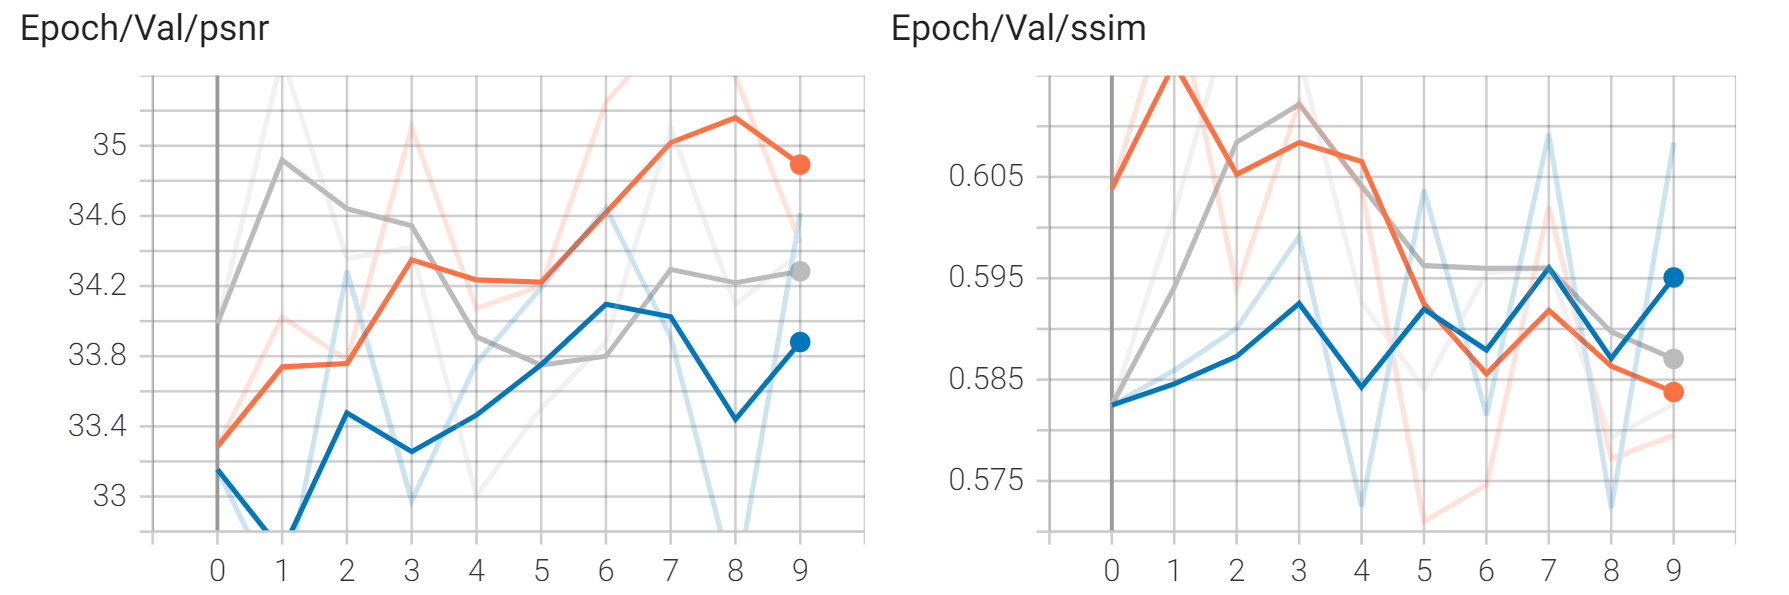
\includegraphics[width=\textwidth, keepaspectratio]{project-val-psnr-ssim-lr.png}
        \caption{PSNR and SSIM values with lr: 0.01 (gray), 0.001 (orange), 0.0001 (blue)}        
    \end{subfigure}
    \caption{Experiments with different \textit{lr}.}\label{project:lr-experiments}
\end{figure}

The initial learning rate is set to \textbf{0.001} based on the experiments done (\Cref{project:lr-experiments}).

\subsubsection{Overfitting}

In order to see if the network was capable to learn the mapping some overfitting experiments were done [\Cref{project:overfitting-experiments}]: neither increasing the epochs (red) nor the complexity of the model(light blue) lead to overfitting with respect to the baseline (dark blue) [\Cref{project:model-overfitting-complexity}].

Moreover the noisy loss could be caused by the regularization action of the small batch size and by training data downsampled using a bilinear interpolation which can be seen as an data augmentation used for generalization and regularization of the network.

An lr scheduler was used in order to try to decrease further the loss but without success (\Cref{project:lr-scheduler-experiments}).


\begin{table}
    \centering
    \makebox[\textwidth]{
        \begin{tabular}{l|ccc}
            & Paper model & Base model(dark blue) & Complex model (light blue) \\
            Total params & 22,405,168 & 828,928 & 1,111,270 \\
            Trainable params & 22,405,168 & 828,928 & 1,111,270 \\
            Non trainable params  & 0 & 0 & 0 \\
            \hline 
            Input size (MB) & 0.84 & 0.84 & 0.84 \\
            Forward/Backward pass size (MB) & 10231.38 & 4911.24 & 5281.37 \\
            Params size (MB) & 85.47 & 3.16 & 4.24 \\
            Estimated total size & 10317.70 & 4915.24 & 5286.45                    
        \end{tabular}
    }    
    \caption{Comparison complexity between models.}\label{project:model-overfitting-complexity}
\end{table}

\begin{figure}[H]
    \begin{subfigure}{\textwidth}
        \centering
        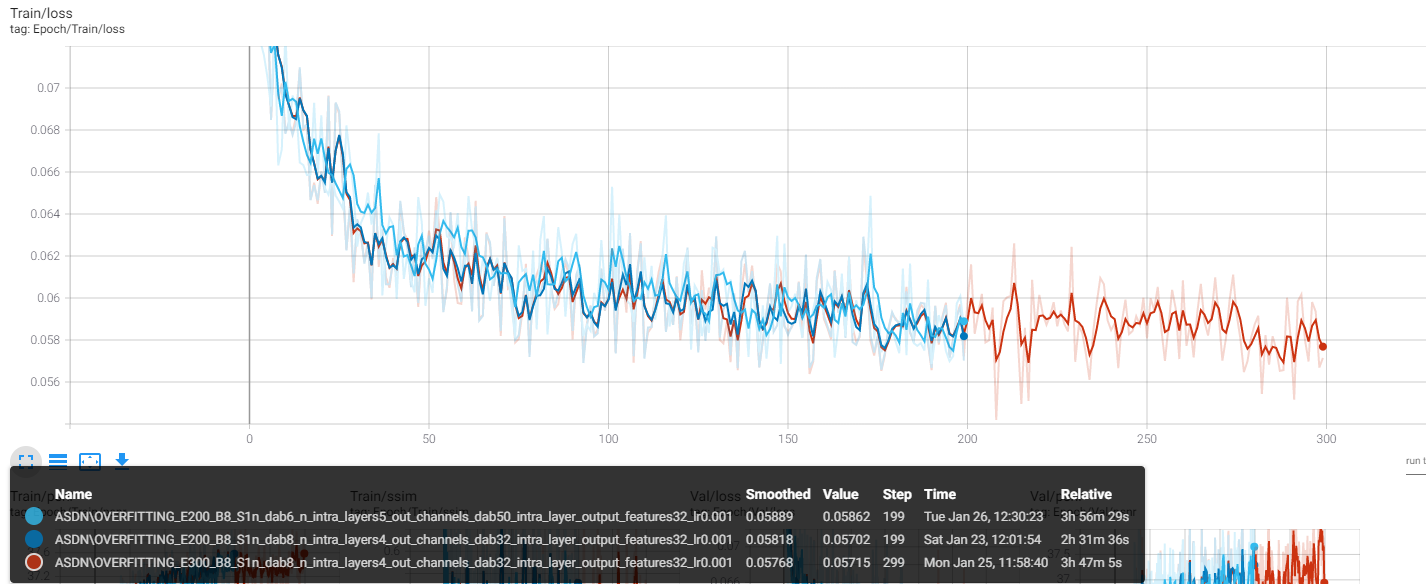
\includegraphics[width=\textwidth, keepaspectratio]{project-overfitting.png}
        \caption{Loss.}        
    \end{subfigure}
    \begin{subfigure}{\textwidth}
        \centering
        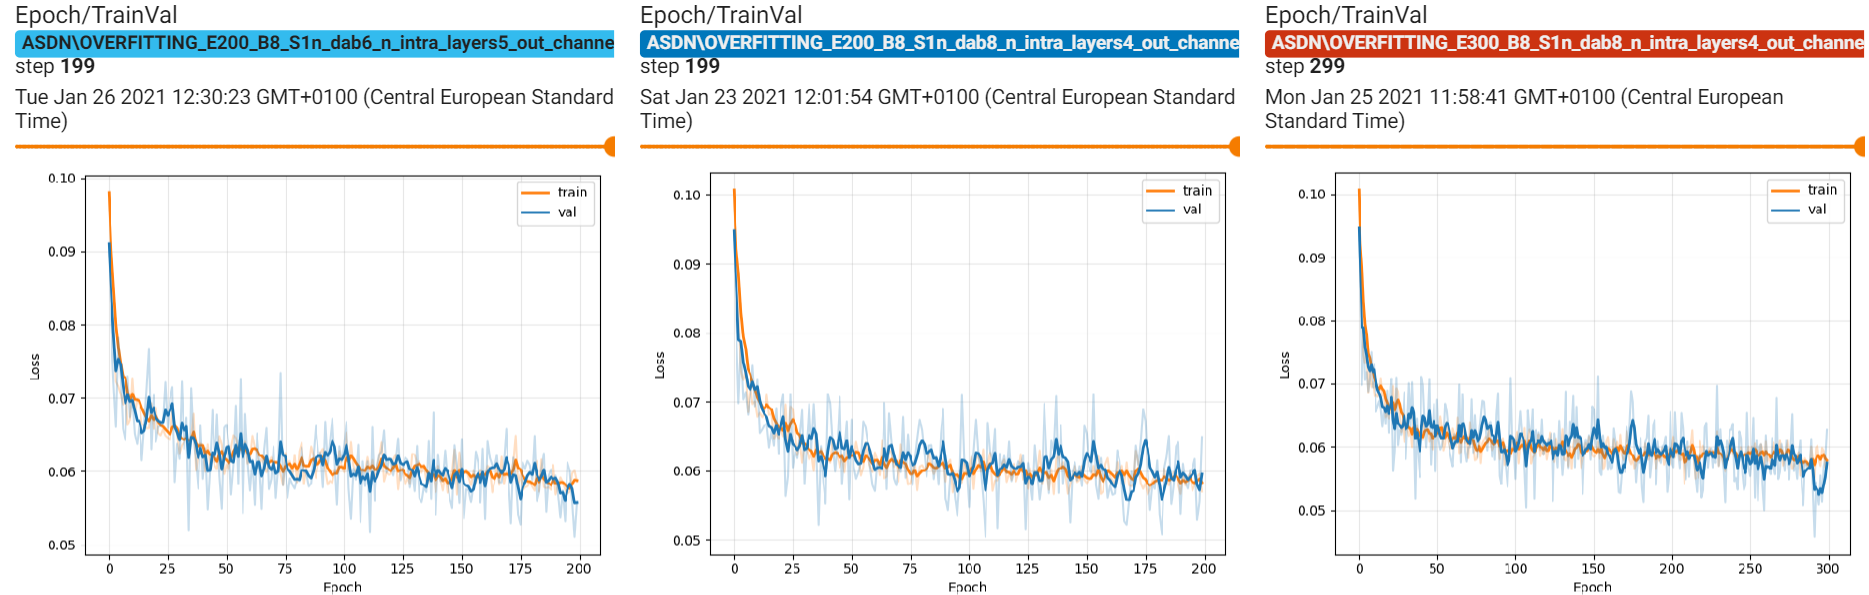
\includegraphics[width=\textwidth, keepaspectratio]{project-overfitting-trainval.png}
        \caption{Train-Val loss.}
    \end{subfigure}    
        \caption{Overfitting experiments.}\label{project:overfitting-experiments}           
\end{figure}

\begin{figure}[H]
    \begin{subfigure}{\textwidth}
        \centering
        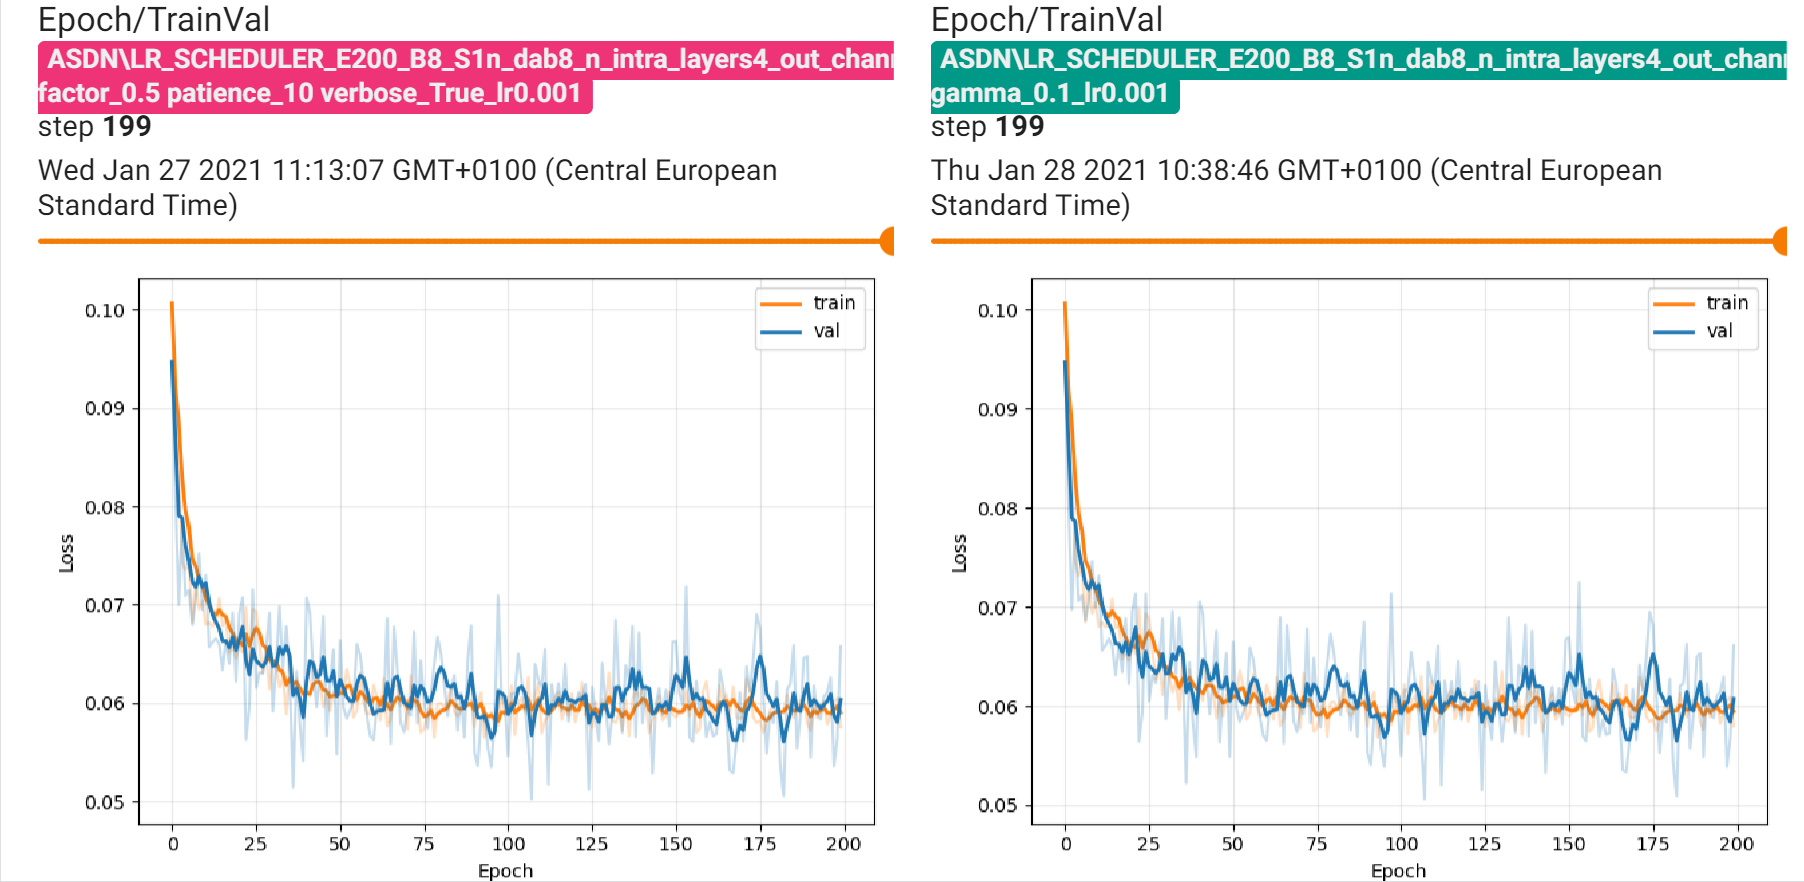
\includegraphics[width=\textwidth, keepaspectratio]{project-lr-scheduler.png}
        \caption{Train-Val loss with StepLR(green) and ReduceLROnPlateau(pink).}
    \end{subfigure}
    \begin{subfigure}{\textwidth}
        \centering
        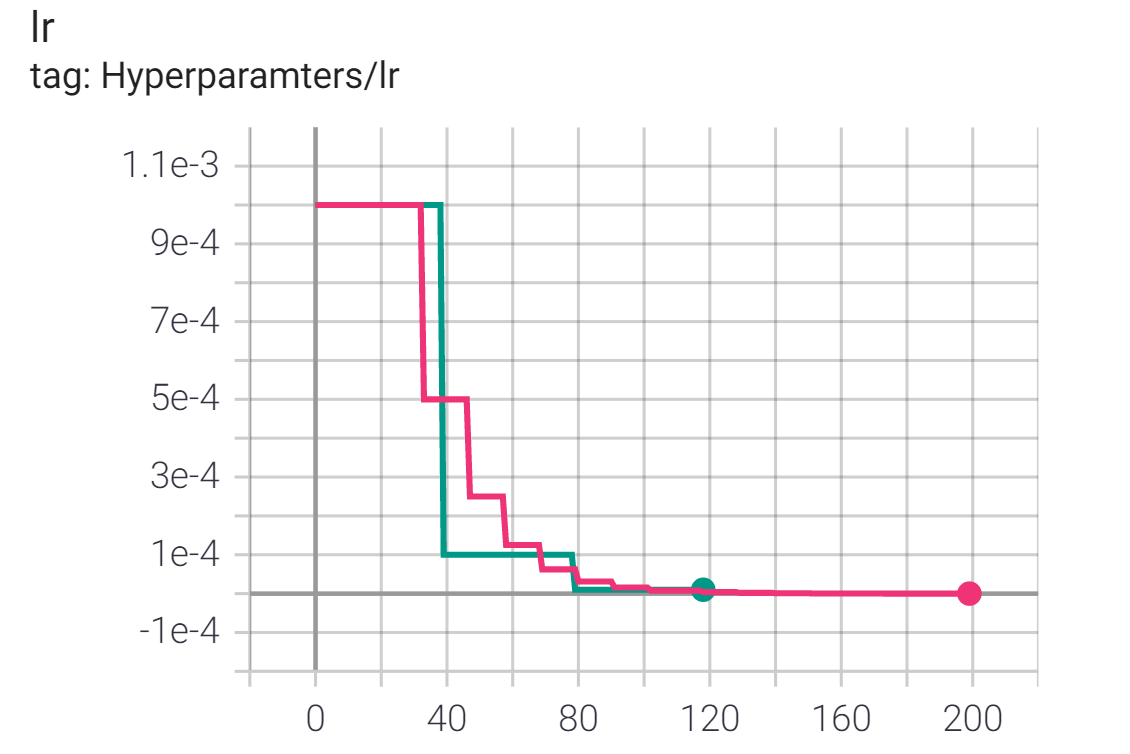
\includegraphics[width=\textwidth, keepaspectratio]{project-lr-scheduler-lr.png}
        \caption{LR trend with StepLR(green) and ReduceLROnPlateau(pink).}
    \end{subfigure}
    \caption{LR scheduler experiments.}\label{project:lr-scheduler-experiments}
\end{figure}

\subsubsection{Training}

The network was trained for 500 epochs without and with data augmentation (random vertical flip, random horizontal flip, random 90 degree rotation) in order to increase patches seen without increasing the number of images and therefore without increasing training time and  aggressively reducing the lr in order to see an improvement of the loss.

In both case the loss is steady to \textasciitilde 0.6 and no real difference between outputs can be seen [\Cref{project:training}] .

\begin{figure}[H]
    \begin{subfigure}{\textwidth}
        \centering
        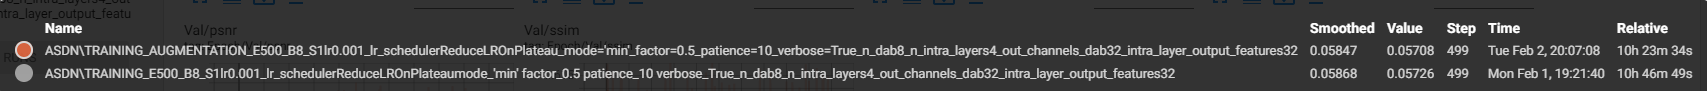
\includegraphics[width=0.9\textwidth, keepaspectratio]{project-training-time.png}
        \caption{Training time.}
    \end{subfigure}
    \begin{subfigure}{\textwidth}
        \centering
        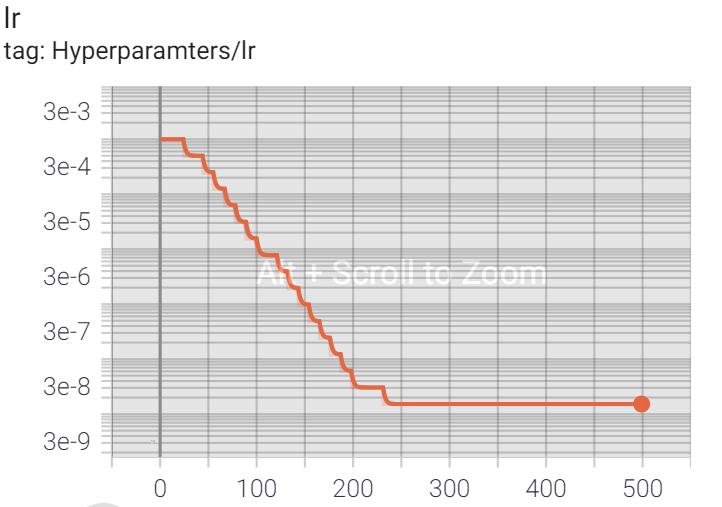
\includegraphics[width=0.9\textwidth, keepaspectratio]{project-training-lr.png}
        \caption{Learning rate over time.}
    \end{subfigure}
    \begin{subfigure}{\textwidth}
        \centering
        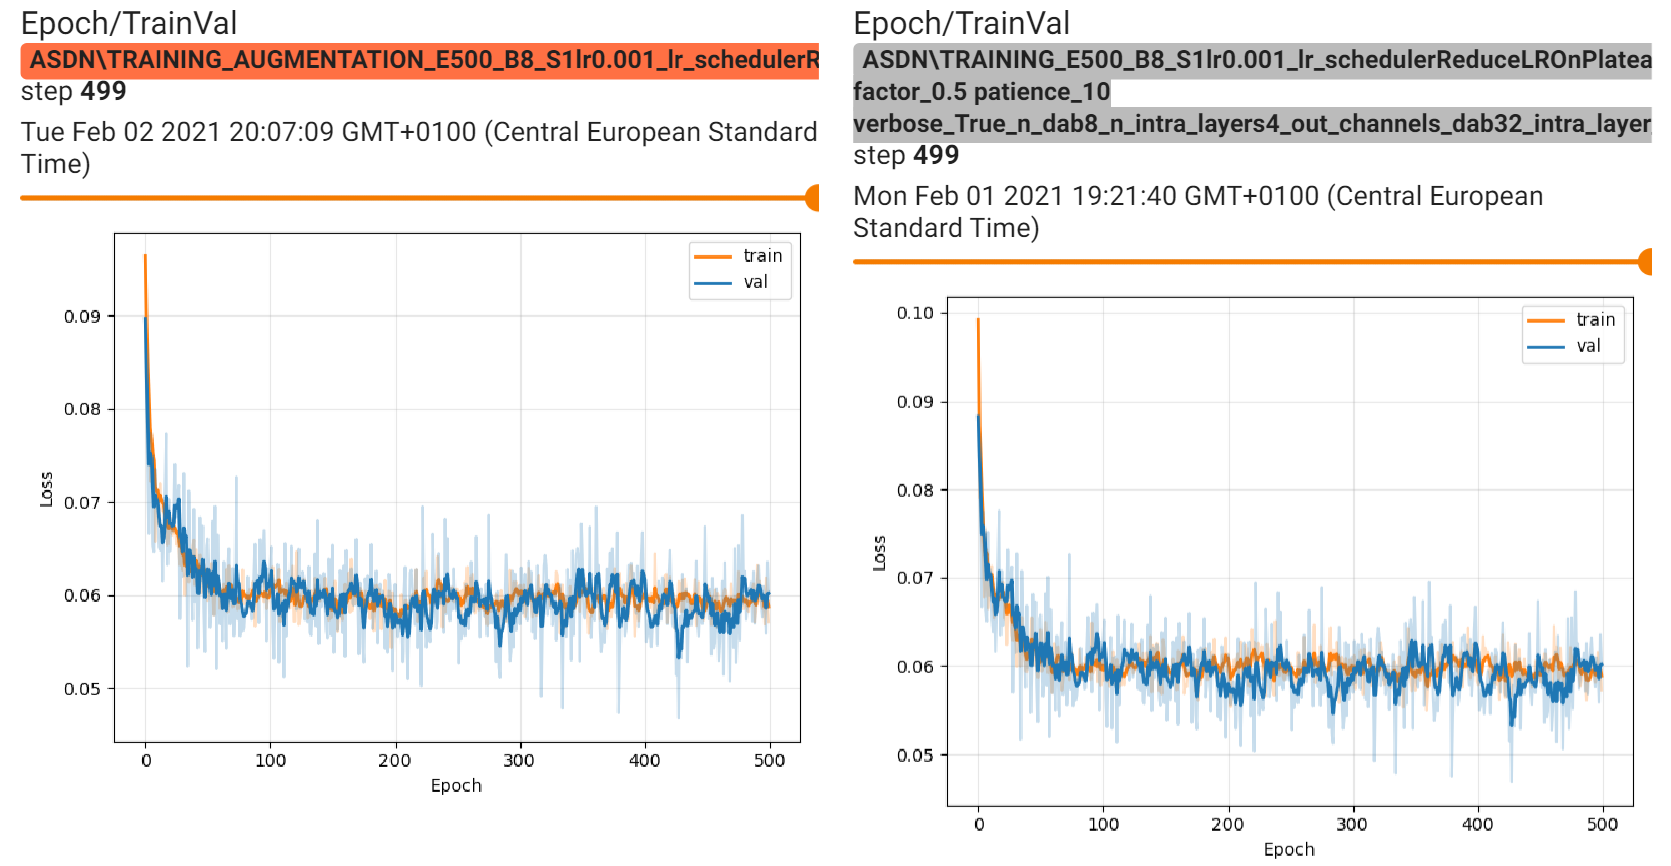
\includegraphics[width=\textwidth, keepaspectratio]{project-training-val-loss.png}
        \caption{Train-Val loss.}
    \end{subfigure}
    \caption{Training with 500 epochs.}
\end{figure}

\begin{figure}[H]
    \begin{subfigure}{\textwidth}
        \centering
        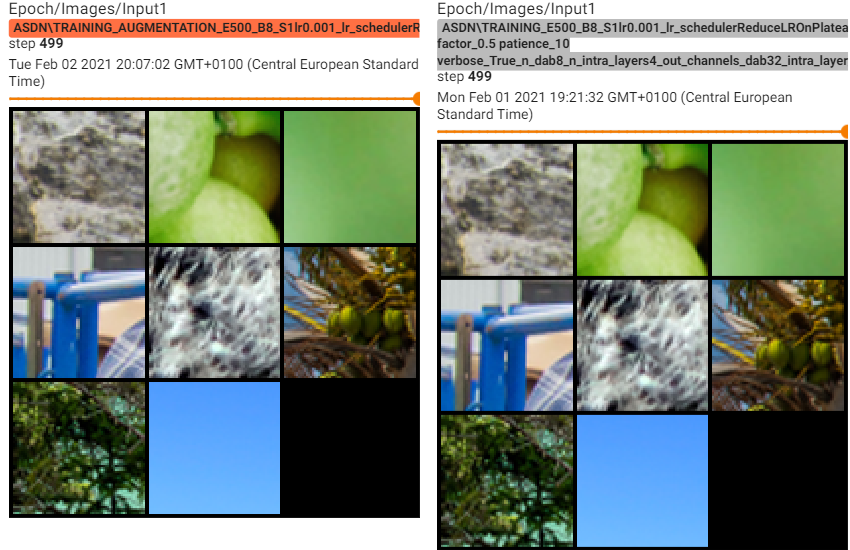
\includegraphics[width=\textwidth, keepaspectratio]{project-input-e500.png}
        \caption{Input.}
    \end{subfigure}
    \begin{subfigure}{\textwidth}
        \centering
        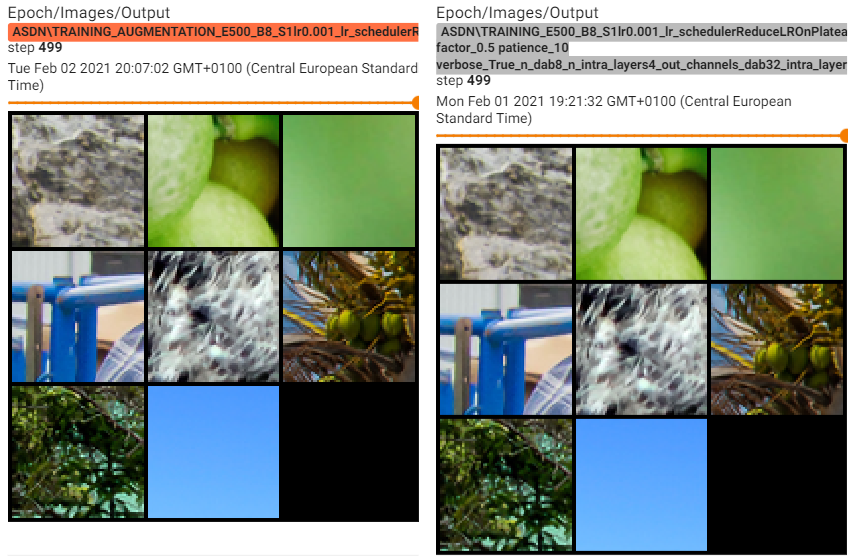
\includegraphics[width=\textwidth, keepaspectratio]{project-output-e500.png}
        \caption{Output.}
    \end{subfigure}
    \caption{Validation images at 500-th epoch.}\label{project:training}
\end{figure}

\subsubsection{Ensemble}
An ensemble was created averaging parameters saved during the training reducing lr with the policy defined in \textit{Snapshot ensembling}\cite{snapshotesembling}.
The lr, loss and val loss of each model at the end of the cycle are:
\begin{figure}[H]
    \centering
    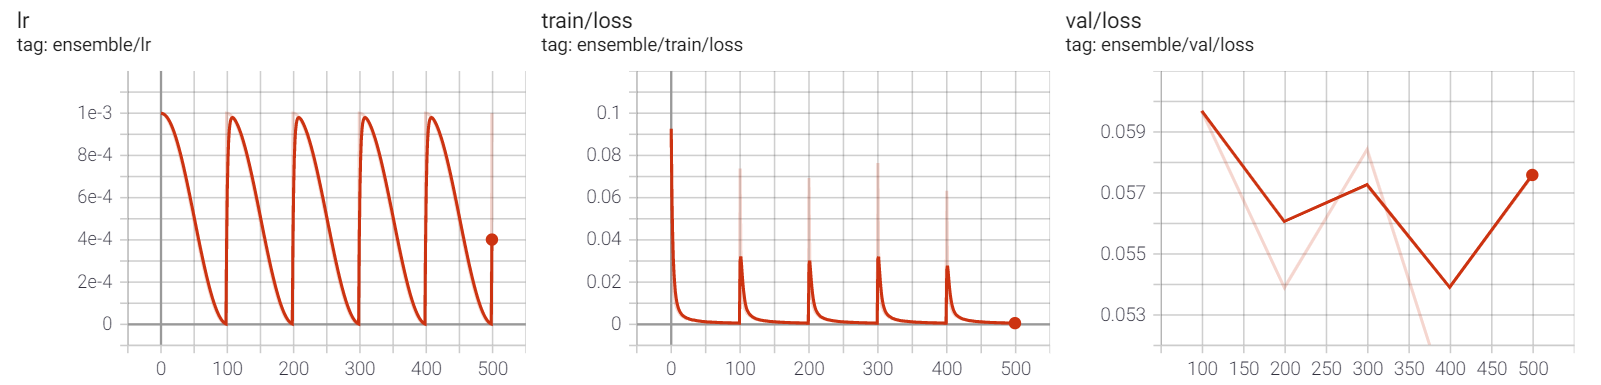
\includegraphics[width=\textwidth, keepaspectratio]{project-ensemble-lr-loss-valloss.png}
    \caption{Learning rate, training loss and validation loss.}
\end{figure}

\subsubsection{Testing}
The following are the results


\begin{table}[H]
    \begin{tabular}{lllll}
    Dataset    & \multicolumn{2}{l}{Base} & \multicolumn{2}{l}{Ensemble} \\
               & PSNR       & SSIM        & PSNR         & SSIM          \\
    BSDS100    & 24.924     & 0.73514     & 24.777       & 0.73414       \\
    Manga109   & 23.306     & 0.82064     & 22.879       & 0.81448       \\
    Set14      & 24.109     & 0.74444     & 23.811       & 0.73910       \\
    Set5       & 26.984     & 0.83924     & 26.699       & 0.83623       \\
    Urban100   & 21.776     & 0.71635     & 21.553       & 0.71324       \\
    historical\footnotemark & 20.675     & 0.66890     & 20.533       & 0.66516      
    \end{tabular}
    \end{table}
\footnotetext{Ground truth images were already LR images}

The only comparison is done with bicubic interpolation. 
The network is able to reconstruct sharp edges but unable to restore all the details from the original image [\Cref{project:test-Urban100},\Cref{project:test-Manga109},\Cref{project:test-Set5},\Cref{project:test-Set14},\Cref{project:test-BSDS100},\Cref{project:test-historical}] although images are a bit less blurred using the ensemble \footnote{In order to see the difference is necessary to jump faster from one image to the other}.

\drawtestimages{Urban100}{project-urban-100}{0.168} %OK
\drawtestimages{Manga109}{project-manga-109}{0.20} %OK
\drawtestimages{Set5}{project-set-5}{0.75} %OK
\drawtestimages{Set14}{project-set-14}{0.43} %OK 
\drawtestimages{BSDS100}{project-bsds-100}{0.52} %OK
\drawtestimages{historical}{project-historical}{0.78} %OK

